\section{\I{The population section}\label{sec:population-section}}

\subsection{Introduction}

The population section\index{Population section} defines the model structure, movement and population dynamics, and other associated parameters. It describes the model structure (both the spatial and population structure), defines the population  (for example, recruitment, migration, and mortality) and movement processes, defines the layers (the known attributes of each spatial cell), selectivities, and model parameters.

The population section consists of several components, including;
\begin{itemize}
  \item The spatial and population structure
  \item Model initialisation (i.e., the state of the model at the start of the first year)\index{Initialisation}\index{Model ! initialisation}
  \item The annual cycle (time steps and processes that are applied in each time step)\index{Annual cycle}
  \item The specifications and parameters of the processes;
  \begin{itemize}
    \item Population processes (i.e., processes that add, remove individuals to or from the partition, or shift numbers between ages and categories in the partition)
    \item Spatial processes (i.e., processes that move or shift cohorts between spatial locations but do not alter their ages or categories)
  \end{itemize}
  \item Layers (used by processes, observations and reports) and their definitions
  \item Selectivities
  \item Parameter values and their definitions
  \item Derived quantities required as parameters for some processes (i.e., spawning stock biomass to resolve the spawner-recruit relationship in a recruitment process)
\end{itemize}

\subsection{\I{Spatial structure}\label{sec:spatial-structure}}

The spatial structure of \SPM\ is represented by an $n_{rows} \times n_{cols}$ grid, with rows $i=1 \dots n_{rows}$ and columns $j=1 \ldots n_{cols}$. Each cell of this matrix records the population structure at that point in space, where the population structure is represented by an $n_{categories} \times n_{ages}$ rectangular matrix (with categories $k=1 \ldots n_{categories}$ and ages $l=1 \ldots n_{ages} = age_{min} \ldots age_{max}$. Hence we can describe any spatial and population element of the model as element$(i,j,k,l)$. We define, within the spatial grid ($n_{rows} \times n_{cols}$), locations where the population can and cannot potentially be present using a \emph{layer}. 

\SPM\ implements a single spatial structure, a grid of \emph{square} cells (Figure \ref{fig:SquareSpatialStructure}) The spatial grid can be of an arbitrary size, but must be rectangular. 

The dimensions of the spatial grid are user defined but must be at least a $1 \times 1$ grid (i.e., a single spatial cell). But the largest spatial structure allowed by \SPM\ is a grid of $1000 \times 1000$ cells\index{Maximum size of the spatial grid}. Associated with the spatial structure is the one compulsory layer (see Section \ref{sec:layers}), the \emph{base layer}\index{Base layer}. This defines the locations where the population can and cannot potentially be present (e.g., in a marine model, the locations associated with the sea and not land) as values within the base layer that are greater than zero. There must be at least one cell in the spatial grid where the population can be present. In addition, the base layer also defines the relative \emph{area}\index{Cell area} of each spatial cell, as used for density calculations within \SPM.

\begin{figure}[htp]
 \centering
  \resizebox{\textwidth}{!}{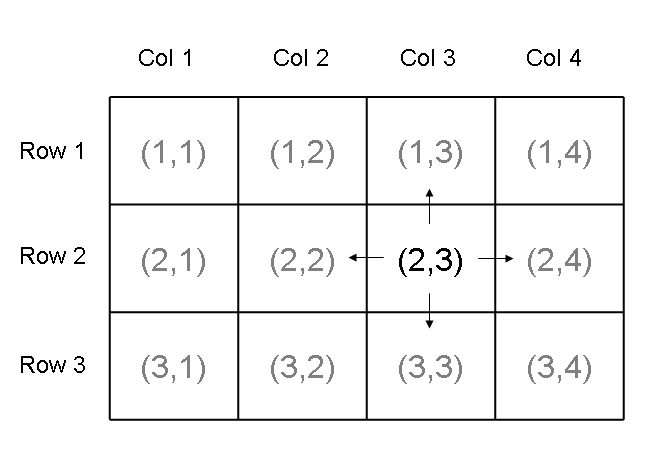
\includegraphics[width=\textwidth]{Figures/SquareStructure}}
  \caption{An illustration of the \emph{square} spatial structure}
  \label{fig:SquareSpatialStructure}
\end{figure}

Models are implemented as a grid of cells as a rectangular matrix. Distance between cells is determined as the euclidean\index{Inter-cell distance} distance between cell centres, modified by an arbitrary scalar. 

Hence, the definition of the spatial structure includes;
\begin{itemize}
\item The type of spatial grid and its dimensions, $n_{rows}$ and $m_{cols}$
\item The label of a numeric layer to be used as the base layer (defining the locations where the population can be present as well as the area of each cell)
\item The length (distance) of a side of the grid cell to be used as the scaler for distance calculations
\end{itemize}

\subsection{\I{Population structure}}

The population structure in \SPM\ is represented by a matrix containing an arbitrary number of user defined categories (rows), and an arbitrary age range (columns). Hence, each spatial cell has a population state described as $n_{categories} \times n_{ages}$ rectangular matrix with categories $k=1 \ldots n_{categories}$ and ages $l=age_{min} \ldots age_{max}$. 

The names and number of categories are user defined, but there must be at least one category defined for a model. The ages are defined as a sequence from $age_{min}$ to $age_{max}$, with the last age optionally a plus group.

Hence, the definition of the population structure includes;
\begin{itemize}
  \item The number and labels of the categories, $k_{categories}$
  \item The minimum and maximum ages that define the ages of the model, $l_{ages}$
  \item If the last age is a plus group
\end{itemize}

\subsection{\I{Layers}\label{sec:layers}}

\emph{Layers} are used by \SPM\ to evaluate locations where the population may be present (via the \emph{base layer}), to provide sets of known attributes of each spatial location (for preference based movements), and to group or categorise cells for use by processes and observations. Layers consist of an $n \times m$ matrix and can be either \emph{numeric} or \emph{categorical}. See Section \ref{sec:population-section} for further details.

Layers form a key underlying concept in \SPM. They comprise of a grid of known values, with a value for every spatial cell in the model. Layers are used by processes, observations, and outputs commands to supply spatially explicit covariates and any categorical groupings required. 

Every model must define at least one layer, the base later $L_B$. A layer is defined as a $n_{rows} \times n_{cols}$ grid of values (with one exception --- the distance layer, see below), where the value for each cell represents a known quantity. For example layers may represent classifications, physical attributes, or some other assumed quantity. Typically they are provided by the user as a matrix of values, although abundance and distance layers can be calculated by \SPM\ as and when required. 

Within \SPM, layers are used in three contexts:
\begin{enumerate}
\item The base layer\index{Base layer}\index{Layers ! the base layer}: The base layer $L_B$ is a special layer (there must be exactly one base layer defined within the model) that defines the locations where the population can and cannot potentially be present (e.g., locations associated with the sea and not land in a marine model). Here, we define that a cell may potentially have part of the population present if every element $L_B(i,j) \ge 0$. Further, positive values of the base layer $L_B$ represent the \emph{area} represented by that spatial cell. 
\item \I{Covariate layers}: A model may have many covariate layers, and these are used as covariates of some population or movement process (e.g., the sea floor depth may be a covariate of some movement process). The values in layers used as covariates must be continuous (i.e., numeric) variables. Covariate layers must have values $\ge0$.
\item \I{Classification layers}. A model may have many classification layers, and these are used as a classification or grouping variable for aggregating data over individual spatial cells $(i,j)$, e.g., statistical areas or management areas. Such layers are typically used to aggregate the population within cells into groups so-as to allow comparison with observations. The values in layers used as classification layers must be categorical.
\end{enumerate}

Typically, layers are supplied by the user and are assumed known and constant. \SPM\ defines the following types of layer;

\begin{enumerate}
\item{\I{Numeric layers}\label{numeric-layer}}: A model may have many numeric layers, and these can be used as covariates of a population or movement process (e.g., depth may be a covariate of some movement process), and/or locations of event mortality. Numeric layers can contain only continuous (numeric) variables. Values for a numeric layer must be supplied for each cell by the user.

\item {\I{Categorical layers}\label{categorical-layer}}: A model may have many categorical layers, and these are used as a classification or grouping variable for aggregating data over individual cells, e.g., management areas. Such layers are typically used to aggregate the population within cells into groups for comparing with observations. The values in layers used as categorical layers can contain any characters (except white space), and are interpreted as categorical values. Values for a categorical layer must be supplied for each cell by the user.

\item {\I{Distance layers}}: A distance layer is one that defines the distance between any two cells. By default, \SPM\ calculates the values of the distance layer as the Euclidean distance (where the grid type is \argument{square}). Here, the distance between cell a and cell b can be defined as,
\begin{equation}
  d(a,b) = \lambda \sqrt{(x_a - x_b)^2 + (y_a - y_b)^2}
\end{equation}
where $x$ and $y$ represent the x- and y-coordinates of $a$ and $b$ respectively, and $\lambda$ is an arbitrary scaler representing the length of one side of the square. Unlike other types of layers, distance layers are not a $n_{rows} \times n_{cols}$ grid of values, but rather a matrix of dimension $(n_{rows} \times n_{cols}) \times (n_{rows} \times n_{cols})$  where the distance between each cell and every other cell is evaluated. Note that under this definition, the distance between any cell and itself is 0. 

\item{\I{Abundance layers}}: The abundance layer is the sum of the number of individuals within cell $a$ in categories $k$ and with selectivity $S_l$ at age $l$. 
\begin{equation}
  N(a) = \sum\limits_{k} \sum\limits_l S_l \ \text{element}(i,j,k,l)
\end{equation}
\SPM\ calculates the values of the layer when running the model at the point in time where the value is required.

\item {\I{Biomass layers}}: The biomass layer \NYI\ is the sum of the biomass of individuals within cell $a$ in categories $k$, with selectivity $S_l$ at age $l$, and mean weight $w_{kl}$
\begin{equation}
  N(a) = \sum\limits_{k} \sum\limits_l w_{k,l} S_l \ \text{element}(i,j,k,l) 
\end{equation}
\SPM\ calculates the values of the layer when running the model at the point in time where the value is required.

\item {\I{Abundance-density layers}}: The abundance density layer is the density of the number of individuals within cell $a$ with area $A_a$ in categories $k$, with selectivity $S_l$ at age $l$,
\begin{equation}
  N(a) = \frac{1}{A_a} \sum\limits_{k} \sum\limits_l S_l \ \text{element}(i,j,k,l)
\end{equation}
\SPM\ calculates the values of the layer when running the model at the point in time where the value is required.

\item {\I{Biomass-density layers}}: The biomass-density layer \NYI\ is the density of the biomass of individuals within cell $a$ with area $A_a$ in categories $k$, with selectivity $S_l$ at age $l$, and mean weight $w_{kl}$,
\begin{equation}
  N(a) = \frac{1}{A_a} \sum\limits_{k} \sum\limits_l w_{k,l} S_l \ \text{element}(i,j,k,l)
\end{equation}
\SPM\ calculates the values of the layer when running the model at the point in time where the value is required.

\item {\I{Meta-layers}\label{meta-layer}}: In addition to the above types of layer, \SPM\ defines a special type of layer known as a \emph{meta-layer} \NYI\. The meta-layer allows individual layers (of the same type) to be indexed by year, and applied as a single layer within the model. For example, assume that we had a model where we wished to use Sea Surface Temperature (SST) as a layer, perhaps to control some movement process. The SST values for each year of the model would be defined as individual numeric layers, each with a unique label. We could then define a meta-layer that indexed the individual annual SST layers by year, and use the meta-layer as the control layer in the movement process.
\end{enumerate}

However, there are  exceptions to this rule --- layers of type biomass, quantity, and distance are calculated automatically by \SPM\ as required. For example, for the distance layer in a square grid, the distance between cell $a$ and cell $b$ is defined as proportional to $\sqrt{(x_a-x_b)^2 +(y_a-y_b)^2}$, where $x$ and $y$ represent the x- and y-coordinates of $a$ and $b$ respectively.

For the abundance layer, the abundance or biomass of a cell is simply a count of the number (or biomass) of individuals in the cell a within categories $K$, with selectivity $S$, e.g., $N(a)=\sum_k \sum_i \ \text{element}(i,j,k,l)$.

Note that \SPM\ does not `edit' or otherwise change layers, including adding or otherwise combining layers that are supplied in the input parameter files.

\subsection{\I{Time sequences}}

The time sequence of the model is defined in three parts;
\begin{itemize}
  \item \I{Initialisation}
  \item \I{Run years}
  \item \I{Projection year}s
\end{itemize}

\subsubsection{\I{Annual cycle}}

The annual cycle is implemented as a set of processes that occur, in a user-defined order, within each year. User-defined time steps are used to break the annual cycle into separate components, and allow observations to be associated with different sets of processes. Any number of processes can occur within each time step, in any order and can occur multiple times within each time step. Note that time steps are not implemented during the initialisation phases, and that the annual cycle in the initialisation phases can be different from that run during the model years.

\subsubsection{\I{Initialisation}}

Model initialisation can occur in several phases\index{Initialisation!phases}, each which iterates through a number of years carrying out the population and/or spatial processes defined for that phase. At the end of the initialisation step, \SPM\ runs through the model years carrying out processes in the order defined in the annual cycle, and can evaluate expected values of observations in order to calculate likelihoods, project forward to determine future states \NYI, or simulate observations from the current state.

\SPM\ initialises the initial equilibrium state as an iterative process, because a general solution that initialises complex structured movement models can be difficult to implement using analytic techniques. However, initialising via iteration for a long-lived species with complex movements can take many iterations, and be slow to run. In \SPM, we allow for user-defined multi-phased initialisation using iteration to allow the user to optimize models for speed. Each phase of the initialisation can involve any number of population and/or movement processes. 

In each initialisation phase, the processes defined for that phase are carried out and used as the starting point for the following phase or, if it is the last phase, then the years that the model is run over. The first phase is always initialised with each element (i.e., each age and category within each spatial cell) set at zero. Note that this means that recruitment processes where the numbers of recruits is based on a stock recruitment or density dependant relationship will likely fail if used in the first phase of an initialisation. 

The multi-phase iteration also allows the user to determine if the initialisation has converged in a particular model run. Here, add an additional initialisation phase for, say, $1$ year as the last initialisation phase (with the same processes applied). Then, using the initialisation reports (\commandlabsubarg{report}{type}{initialisation\_phase}), print a copy of the partition just before and just after that phase. If the initialisation has converged to an equilibrium state, then the partition at both these time intervals will be the same.

Hence, for initialisation you need to define;
\begin{itemize}
  \item The initialisation phases
  \item The number of years in each phase and the processes to apply in each
\end{itemize}

\subsubsection{\I{Model years}}

Following initialisation, the model then runs over a number of user-defined years. For this part of the model, the annual cycle can be broken into separate time steps, and observations can be associated with the state of the model at the end of any time step, i.e., likelihoods for particular observations are evaluated, if required, at the end of each time step. 

Processes are carried out in the order specified within each time step, and can be the same or different to processes in other initialisation phases of the model. The run years define the years over which the model is to run and the annual cycle within each year. The model runs from the start of year \argument{initial} and runs to the end of year \argument{current}. The projection part \NYI\ then extends the run time up to the end of year \argument{final}. 

\begin{itemize}
  \item The time steps and the processes applied in each
  \item The initial year (i.e., the model start year)
  \item The current year (i.e., the model end year)
  \item The final year (i.e., the model projection end year)
\end{itemize}

\subsubsection{\I{Projections}\label{sec:projections}}

\SPM can project, from a set of parameter estimates, the state of the model into the future \NYI. In a projection run, the model is initialised and run through the model years from \argument{initial} to the \argument{current}. Then, the partition is run from \argument{current} to \argument{final}. 

\subsection{\I{Processes}}

Processes produce changes in the model partition, by adding, removing or moving individuals between spatial cells (movement processes), and ages or categories (population processes). These include processes such as recruitment, mortality, ageing, and various forms of movement.

\SPM\ has two types of processes, \emph{population}\index{Population processes} and \emph{movement}\index{Movement processes} processes. Population processes are those processes which modify, move or otherwise change the numbers of individuals \emph{within} a spatial cell, i.e., they do not affect the spatial location of a cohort. Movement processes, on the other hand, move, shift or otherwise modify cohorts \emph{between} spatial cells, but do not affect the age or category of the numbers in each cohort. 

The population processes include recruitment\index{Recruitment}, ageing\index{Ageing},  mortality\index{Mortality} events (e.g., natural and exploitation) and category transition processes\index{Category transition} (i.e., processes that move individuals between categories, while preserving their age structure). See Section \ref{sec:population-section} for a complete list of available processes.

Each of these processes is carried out in the user-defined prescribed order when initialising the model, and then for a user-defined order in each year in the annual cycle\index{Annual cycle}.

\SPM\ implements three different types of movement processes\index{Movement};
\begin{enumerate}
	\item  A migration movement rate\index{Migration} of cohorts between any two locations, and is roughly analogous to movements between areas as implemented in other population models, such as CASAL \citep{1388}. \NYI
	\item An adjacent cell movements\index{Adjacent cell movement}, parametrised by some function of an underlying layer --- equivalent to, for example, movement processes implemented in Fish Heaven \citep{1136,1135}. \NYI
	\item Movement parametrised as a probability density function\index{Preference movement}. Here, the key underlying idea is that the spatial distribution of cohorts at any point in time and at any location can be represented as a density function based on attributes of that location, local abundance, and/or distance from their previous location \citep{1366,1367}. 
\end{enumerate}

An \SPM\ model can be parametrised by both population processes (for example, ageing, recruitment, and mortality), and movement processes. Population processes are those processes which modify, move or otherwise change the numbers of individuals within a spatial cell, i.e., they do not affect the spatial location of a cohort. Movement processes, on the other hand, move, shift or otherwise modify cohorts between spatial cells, but do not affect the age or category of the numbers in each cohort. 

\subsection{\I{Population processes}}

Population processes are those processes that change the population state of individuals, but retain their location. The population processes are described below.

\subsubsection{\I{Recruitment}}

Recruitment processes are defined as  process that introduces new individuals into the model. \SPM\ implements two types of recruitment process, constant recruitment\index{Recruitment ! Constant} and \I{Beverton-Holt recruitment}\index{Recruitment ! Beverton-Holt} \citep{1203}. 

In both of the recruitment process, a number of individuals are added to the partition at the age and categories specified. If more than one category is defined, then the proportions of individuals added across categories are user-defined. For example, if recruiting to categories labelled male and female, then you might set the proportions as $0.5$ and $0.5$ respectively to denote that half of the recruits recruit to the male category and the remaining half to the female category.

For each cell where cell$(i,j)$ is a member of some layer $L_R$, the  number of fish added in year $y$ is 
\begin{equation}
  \text{element}(i,j,k,l) \leftarrow \text{element}(i,j,k,l) + p_k(R_y / n) \frac{L_ij}{\sum_ij L_ij}
\end{equation}

where age is the age defined as the recruitment age, $p_k$ is the proportion recruitment to category $k$ defined to have recruitment, $n$ is the number of spatial locations where recruitment occurs, and the recruitment to each cell is scaled to be proportional to the value of the layer in that cell.

In the constant recruitment process, $R_y$, the number of recruits in year $y$ is simply the average recruitment $R_0$, i.e.,
\begin{equation}
  R_y = R_0
\end{equation}

For example, to specify a constant recruitment process, where individuals are added to the category `immature' at $age=1$, and the number to add is $R_0=5 \times 10^5$ in areas proportional to the value of the layer \texttt{recruitment}, then the syntax is,

\begin{verbatim}
@process Recruitment
type constant_recruitment
categories immature
proportions 1.0
R0 500000
ages 1
layer recruitment
\end{verbatim}

In the Beverton-Holt recruitment process, $R_y$, the number of recruits in year $y$ is the product of the average recruitment $R_0$, the annual year class strength multiplier, $YCS$, and the stock-recruit relationship i.e.,
\begin{equation}
  R_y = R_0 \times YCS_{y-offset} \times SR(SSB_{y-offset})
\end{equation}

where $offset$ if the number of years offset to link the year class with the year of spawning, and $SR$ is the Beverton-Holt stock-recruit relationship, parametrised by the steepness, $h$,
\begin{equation}
SR(SSB) = \frac{SSB}{B_0} / \left( 1-\frac{5h-1}{4h} \left( 1-\frac{SSB}{B_0} \right) \right)
\end{equation}

Note that the Beverton-Holt recruitment process requires a value for $SSB$ to resolve the stock-recruitment relationship. Here, a derived quantity (see Section \ref{sec:derived-quantities}) must be defined that provides the $SSB$ for the recruitment process.

\subsubsection{\I{Ageing}\label{sec:ageing}}

The ageing process simply moves all individuals in the named categories to the next age class. The ageing process is defined as,
\begin{equation}
  \text{element}(i,j,k,l) \leftarrow \text{element}(i,j,k,l-1)
\end{equation}

except that in the case of the plus group (if defined), 
\begin{equation}
  \text{element}(i,j,k,age_{max}) \leftarrow \text{element}(i,j,k,age_{max}) + \text{element}(i,j,k,age_{max-1}).
\end{equation}

For example, to apply ageing to the categories \texttt{immature} and \texttt{mature}, then the syntax is,

\begin{verbatim}
@process Ageing
type ageing
categories immature mature
\end{verbatim}

Note that ageing is \emph{not} applied by \SPM\ by default. As with other processes, \SPM\ will not apply ageing unless its defined and specified as a process within the annual cycle. Hence, it is possible to specify a model where a category is not aged. \SPM\ will not check or otherwise warn if there is a category defined where ageing is not applied.

\subsubsection{\I{Mortality}\label{sec:mortality}}

Four types of mortality processes are permissible in \SPM, constant, annual-rate \NYI, event, or biomass-event \NYI. These processes remove individuals from the partition, either as a rate (for constant or annual-rate), or as a total number (abundance) or biomass of individuals (for event or biomass-event). \SPM\ does not (yet) implement the Baranov catch equation or any other process where both natural and event mortality are applied simultaneously. To approximate concurrent natural and event mortality, the population processes must be defined to remove some natural mortality (e.g., as a constant or annual-rate), then some event mortality in sequence. It is up to the user to specify how this happens.

Mortalities as rates can depend on a layer. Here only one method of dependence is implemented, the multiplicative method. The multiplicative natural mortality method defines that the value of instantaneous mortality applied to the population state within each cell is the product of the layer value, a selectivity-at-age, and the mortality rate. 

For example, let the mortality rate applied to the population at cell $a$ in category $k$ and age $l$ be denoted $M(a,k,l)$, and given a value from a layer $L_a$  at $a$, a constant morality rate $M$, and a selectivity-at-age $S_l$ at age $l$ for some user-defined categories $k$ then, 
\begin{equation}
  M(a,k,l) = ML_a S_l 
\end{equation}

And the resulting number of individuals remaining in cell $a$ in category $k$ at age $l$ from applying the constant mortality process is,
\begin{equation}
  n'(a,k,l) = n(a,k,l) \exp \left({-M(a,k,l)}\right)
\end{equation}

Mortality for the annual rate is similar, except that the rate applied in each year is defined as a separate value. 

For example, to specify an constant annual mortality rate ($M=0.2$) for categories `immature' and `mature', then, 

\begin{verbatim}
@process NaturalMortality
type constant_mortality_rate
categories immature mature
M 0.2 0.2
selectivities One One
\end{verbatim}

Note that the mortality rate process requires a selectivity. To apply the same mortality rate over all age classes, use a selectivity defined as $S_i=1.0$ for all ages $i$, e.g.,

\begin{verbatim}
@selectivity One
type constant
c 1
\end{verbatim}

The event mortality types\index{Event mortality} act in a similar manner, except that it removes a specified abundance (number of individuals) or biomass from the partition, rather than applying a mortality rate. However, the maximum abundance or biomass to remove is constrained by a maximum exploitation rate.

The event mortality types must be defined using a layer. Here, the abundance or biomass to remove from a the population for each cell $a$ is the value of the layer at $a$ (denoted $F_a$) --- except where there are too few individuals for the event mortality to be taken (as defined by the maximum exploitation rate). In this scenario, \SPM\ removes as many individuals or as much biomass as it can while not exceeding the maximum exploitation rate. Event mortality processes require a penalty function to discourage parameter values that do not allow a the defined number of individuals to be removed. Here, the model penalises those parameter estimates that result in an insufficient number of individuals in defined categories (after applying selectivities). See Section \ref{sec:penalties} for more information on specifying penalties.

For example, the event mortality applied to user-defined categories $k$, with the numbers removed at age $l$ determined by a selectivity-at-age $S_l$ is applied as follows:

First, calculate the vulnerable abundance for each category $k$ in $1 \ldots K$ for ages $l = 1 \ldots L$ that are subject to event mortality,
\begin{equation}
  V(k,l) = S(l) N(k,l)
\end{equation}

And hence define the total vulnerable abundance $V_{Total}$ as,
\begin{equation}
  V_{Total}  = \sum\limits_K {\sum\limits_L {V(k,l)}} 
\end{equation}

Hence the exploitation rate\index{Maximum exploitation rate} to apply is 
\begin{equation}
U = \begin{cases}
  C/V_{total}, & \text{if $C/V_{total} \leq U_{max}$} \\
  U_{max}, & \text{otherwise}\\ 
  \end{cases} 
\end{equation}

And the number removed $R$ from each age $l$ in category $k$ is,
\begin{equation}
  R(k,l) = UV(k,l)
\end{equation}

For example, to specify fishing mortality based on spatially explicit catches (and given for each year as a layer, `Catch2000', `Catch2001', etc,.) over categories `immature' and 'mature' with selectivity `FishingSel' and assuming a maximum possible exploitation rate of 0.7, then the syntax is,

\begin{verbatim}
@process Fishing
type event_mortality
categories immature mature
years 2000 2001 2002
layers Catch2000 Catch2001 Catch2002
U_max 0.70
selectivities FishingSel FishingSel FishingSel
penalty event_mortality_penalty
\end{verbatim}

%Similarly, the biomass-event mortality type is applied as \ldots \textbf{to be added}.

\subsubsection{\I{Category transition}s}

Category transition processes move individuals between categories. \SPM\ implements two types, the total number and a rate. 

The category transition process moves a number $n$ between some source and sink category (or categories). This process may be used, for example, to implement a 'tagging' process for mark-recapture data. We define the transition process with selectivity $S$ for source category $a$ and sink category $b$ as,

\begin{equation}\begin{split}
  & \text{element}(i,j,a,l) \leftarrow \text{element}(i,j,a,l) - \frac{nS_l}{\sum\limits_l S_l} \times \text{element}(i,j,a,l) \\
  & \text{element}(i,j,b,l) \leftarrow \text{element}(i,j,b,l) + \frac{nS_l}{\sum\limits_l S_l} \times \text{element}(i,j,a,l)
\end{split}\end{equation}

Category transition processes require a penalty function to discourage parameter values that do not allow a the defined number of individuals to be moved. Here, the model penalises those parameter estimates that result in an insufficient number of individuals in the source category (after applying the selectivity) available to be moved. See Section \ref{sec:penalties} for more information on specifying penalties.

If multiple categories of sources or sinks are defined, then they must be defined in `pairs'. The proportions of selected individuals in the source categories is used to define the proportions of individuals `moved' to the sink categories, as defined by the order that they are specified. For example, to `tag' a population of immature and mature individuals, , then you might define a category transition process \texttt{tagging} with selectivities \texttt{tagging-Sel}, as,

\begin{verbatim}
@process tagging
type category_transition
from immature mature
selectivities tagging-Sel tagging-Sel
to immature-tag mature-tag
years 2001 2002 2003
layers TagRelease2001 TagRelease2002 TagRelease2003
penalty tag_release_penalty
\end{verbatim}

Note that this syntax can be used to combine individuals, simply by repeating a category label when specifying the sink categories.

The transition rate type moves a proportion $p$ between a source and sink category. The transition rate process with selectivity $S$ for source category $a$ and sink category $b$ is,
\begin{equation}\begin{split}
  & \text{element}(i,j,a,l) \leftarrow \text{element}(i,j,a,l) - pS_l \times \text{element}(i,j,a,l) \\
  & \text{element}(i,j,b,l) \leftarrow \text{element}(i,j,b,l) + pS_l \times \text{element}(i,j,a,l)
\end{split}\end{equation}

If multiple categories of sources or sinks are defined, then they must be defined in `pairs'. \SPM\ treats each pair of categories as an independent transition --- but note that these are applied in order that they are specified. For example, to `mature' males and females in a model with four categories \texttt{male-immature}, \texttt{female-immature}, \texttt{male-mature}, and \texttt{female-mature}, then you might define a category transition process \texttt{maturation} with selectivities \texttt{male-maturity} and \texttt{female-maturity}, as,

\begin{verbatim}
@process maturation
type category_transition_rate
from male-immature female-immature
to male-mature female-mature
proportions 1.0 1.0
selectivities male-maturity female-maturity
\end{verbatim}

Note that this syntax can be used to combine individuals, simply by repeating a category label when specifying the sink categories. Similarly, individuals within a category can be split into more than one category by repeating a category label when specifying the source categories.

\subsection{\I{Movement processes}}

Movement processes are those processes that move individuals between cells but retain the their population state, and are defined such that,
\begin{equation}
\text{element}(i,j,k,l)\leftarrow \text{element}(i,j,k,l) + p \times \text{element}(i',j',k,l)
\end{equation}

i.e., each element in cell$(i,j)$ is updated as the sum of itself and some proportion $p$ of a neighbouring element in cell$(i',j')$. To conserve abundance we also update element$(i',j',k,l)$ as,
\begin{equation}
\text{element}(i',j',k,l)\leftarrow \text{element}(i',j',k,l) - p\times \text{element}(i',j',k,l)
\end{equation}

\SPM\ assumes that each movement process occurs simultaneously over all cells (synchronous updating), i.e., all cell updates from each individual movement process are first evaluated for all cells, and then applied to all cells affected. 

\SPM\ implements three types of movement\index{Movement};
\begin{enumerate}
	\item  A migration movement rate of cohorts between any two locations, and is roughly analogous to movements between areas as implemented in other population models, such as CASAL \citep{1388}. 
	\item An adjacent cell movements, parametrised by some function of an underlying layer --- equivalent to, for example, movement processes implemented in Fish Heaven \citep{1136,1135}.
	\item Movement parametrised as a probability density function. Here, the key underlying idea is that the spatial distribution of cohorts at any point in time and at any location can be represented as a density function based on attributes of that location, local abundance, and/or distance from their previous location \citep{1366,1367}. 
\end{enumerate}

\subsubsection{\I{Migration movement}}

The migration process \NYI\ moves individuals from one location to another. A migration can involve one or more categories and movement at age is defined as some proportion multiplies by a selectivity. Migrations are limited in scope to move individuals from one cell to another, and are available to allow compatibility with limited space models such as CASAL \cite{1388}.

\subsubsection{\I{Adjacent cell movement}}

The adjacent cell movement \NYI\ simply moves a proportion of individuals to neighbouring cells. It can be applied to a limited range of spatial locations by associating it with a layer.

\subsubsection{\I{Preference movement}}

Preference movements allows movement from any $cell(a) \rightarrow cell(b)$, for $\forall a,b \in L_B$ and is implemented as a function of the product of up to $n$ independent \emph{preference functions}. We define the probability of moving from any cell $a$ to any cell $b$, for all $a,b \in L_B$, as a function of the relative preference for that cell. Here, we use the term \emph{preference function}\index{Preference function} \citep{1366,1367} to describe the movement probability distributions. We assume that the population and spatial extent are defined, and that there is a preference function that is a function of some (typically estimable) parameters and a spatially explicit set of known attributes.The preference function movement process allows the number of parameters describing movement to to reduced, and results in a movement process that is some function of some underlying property of each location. For example, if we assume that movement between areas was a function of the Euclidean distance between areas, we could model movement between any two areas as a linear decay or exponential decay function \citep{1366}. Alternately, if distribution and density were correlated with bathymetric depth for a marine organism, we might model the movement and distribution as a function of depth. 

\subsubsection*{The total preference function\index{Total preference function}}

Movement in \SPM\ can be defined as a probability distribution based on an underlying preference function. Here, we define the preference for a cell $x$ as the preference function $f_x(\theta_x,P(x))$, where $\theta_x$ are the parameters for $f_x$. So, given a set of $n$ attributes for cell $x$, we can define a preference function for each, and hence we define the aggregated or total preference function for any cell $x$ as the weighted product of individual preference functions,
\begin{equation}
  P_x=f_1(\theta_1,P_1(x))^{\alpha_1} + f_2(\theta_2,P_2(x))^{\alpha_2} + f_3(\theta_3,P_3(x))^{\alpha_3} + \cdots + f_n(\theta_n,P_n(x))^{\alpha_n}
\end{equation}

where $\alpha_i$ is an arbitrary weighting factor for attribute $i$.

Then we define the probability of moving from cell $a$ to any cell $b$ (where $b$ is defined as the set of all possible cells, including $a$),
\begin{equation}
  p(a\rightarrow b) = \frac{P_a}{\sum\limits_{i \in \forall b} P_i}
\end{equation}

Note that there are three forms of preference function,
\begin{enumerate}
\item Those that are a function of some underlying attribute of a cell, as defined by some arbitrary layer $L$
\item Those that are a function of the abundance (perhaps with a selectivity and for a subset of all categories) of each cell
\item Those that are a function of the distance between the sink and the source cells. 
\end{enumerate} 

Preference functions of the first type are determined only by the parameters of the preference function and some underlying, fixed, attribute. Preference functions of the others are dynamic, i.e. they depend on the relative locations of the cells or on the density of a cell at a particular point in time.

\subsubsection*{Preference functions\index{Preference function}}

Preference functions in \SPM\ include constant, Normal, double-Normal, logistic, inverse-logistic, Exponential, and threshold. These are defined as,

\begin{enumerate}
\item The constant preference function\index{Constant preference function}\index{Preference function ! Constant} has dependent variable $x$ and has no parameters, and is defined as,
\begin{equation}
f(x)=x$, where $0 \leq x \leq 1
\end{equation}

\item The Normal preference function\index{Normal preference function}\index{Preference function ! Normal} has dependent variable $x$ and parameters $\theta = (\mu,\sigma)$, and is defined as, 
\begin{equation}\
f(x | \mu, \sigma) = 2^{-[(x- \mu)/\sigma ]^2} 
\end{equation}
 
\item The double-Normal preference function\index{Double-normal preference function}\index{Preference function ! Double-Normal} has dependent variable $x$ and parameters $\theta=(\mu,\sigma_L,\sigma_R)$, and is defined as,
\begin{equation}
  f(x | \mu, \sigma_L, \sigma_R) = \begin{cases}
    2^{-[(x- \mu)/\sigma_L ]^2}, & \text{if $x \leq \mu$} \\
    2^{-[(x- \mu)/\sigma_R ]^2}, & \text{if $x \ge \mu$}\\
  \end{cases}
\end{equation} 

\item The Logistic preference function \index{Logistic preference function}\index{Preference function ! Logistic} has dependent variable $x$ and parameters $\theta = (a_{50},a_{to95})$, and is defined as,
\begin{equation}
  f(x | a_{50}, a_{to95}) = 1 / [1+19^{(a_{50}-x)/a_{to95}}]
\end{equation}

\item The inverse-Logistic preference function\index{Inverse-Logistic preference function}\index{Preference function ! Inverse-Logistic} has dependent variable $x$ and parameters $\theta = (a_{50},a_{to95})$, and is defined as,
\begin{equation}
  f(x | a_{50}, a_{to95}) =1- 1 / [1+19^{(a_{50}-x)/a_{to95}}]
\end{equation}

\item The Exponential preference function\index{Exponential preference function}\index{Preference function ! Exponential} has dependent variable $x$ and parameters $\theta = (\lambda)$, and is defined as,
\begin{equation}
  f(x | \lambda) =\exp(-\lambda x), \text{where $x \geq 0$ and $0$ otherwise}
\end{equation}

\item The threshold preference function\index{Threshold preference function}\index{Preference function ! Threshold} has dependent variable $x$ and parameters $\theta = (N,\lambda)$, and is defined as,
\begin{equation}
  f(x | N, \lambda) = \begin{cases}
    1, & \text{if $0 \le x \leq N$} \\
    1/\left({\frac{x}{N}}^\lambda\right), & \text{if $x \ge N$}\\
    0, & \text{otherwise}
  \end{cases}
\end{equation}

\end{enumerate}

\subsection{\I{Derived quantities}\label{sec:derived-quantities}}

Derived quantities are values, calculated by \SPM\ as required, that have a single value for each year of the model. Derived quantities can be calculated as either an abundance or as a biomass. Derived quantities are simply the count or sum of cells within some categories, after applying a selectivity, within cells defined by a layer.

Some processes require, as arguments, a population value derived from the population state. These are termed \emph{derived quantities}. For example, a recruitment process may require the amount of spawning stock biomass to resolve the stock-recruit relationship. In this example, the spawning stock biomass could be defined as the abundance or biomass of a part of the population at some point in the annual cycle, for selected ages and categories. Derived quantities are described further in the population section (Section \ref{sec:population-section}).

For example, to define a derived quantity (say spawning stock biomass, SSB) for a model, evaluated at the end of the first time step over areas defined by a layer as the spawning ground but counting all `mature' individuals, we might use the syntax,

\begin{verbatim}
@derived_quantity SSB
categories mature
selectivity One
time_step 1
layer spawning_ground
\end{verbatim}

\subsection{\I{Size-age relationship}\label{sec:size-at-age}}

Size-age relationships \NYI\ are used to determine length frequencies, and hence derive a  weight-at-age (in conjunction with the size-weight relationship) of individuals at age/category. There are two alternative growth curves in \SPM, 

\begin{description}
\item{von Bertalanffy}\index{von Bertalanffy growth curve} where size at age is defined as,
\begin{equation} 
\bar{s}(age)= L_\infty \left( 1 - \exp \left( -k \left(age-t_0 \right) \right) \right)
\end{equation}

\item{Schnute}\index{Schnute growth curve} where size at age is defined as,
\begin{equation}
\bar{s}(age)=\displaystyle\begin{cases}
  \left[ y_1^b + (y_2^b - y_1^b) \dfrac{1-\exp \left(-a(age - \tau_1) \right)}{1-\exp \left(-a(\tau_2 - \tau_1) \right)} \right]^{1/b}, & \text{if $a\ne0$ and $b\ne0$} \\
  \AddVspace
  y_1 \exp \left[ \ln \left( y_2 / y_1 \right) \dfrac{1-\exp \left(-a(age - \tau_1) \right)}{1-\exp \left(-a(\tau_2 - \tau_1) \right)} \right], & \text{if $a\ne0$ and $b=0$} \\
  \AddVspace
  \left[ y_1^b + \left( y_2^b - y_1^b \right) \dfrac{age-\tau_1}{\tau_2 - \tau_1} \right]^{1/b}, & \text{if $a=0$ and $b\ne0$} \\
  \AddVspace
  y_1 \exp \left[ \ln \left( y_2/y_1 \right) \dfrac{age-\tau_1}{\tau_2 - \tau_1} \right] , & \text{if $a=0$ and $b=0$} \\
  \end{cases}
\end{equation}
\end{description}

The von Bertalanffy curve is parameterised by $L_\infty$, $k$, and $t_0$; the Schnute curve \citep{836} by $y_1$ and $y_2$, which are the mean sizes at reference ages $\tau_1$ and $\tau_2$, and $a$ and $b$ (when $b=1$, this reduces to the von Bertalanffy with $k=a$). 

The model can incorporate changes in size-at-age during the year (i.e., growth between fish birthdays) by specifying the growth proportions for each time step of the annual cycle.

\subsection{\I{Size-weight relationship}\label{sec:mean-weight}}

The size-weight relationship \NYI, with parameters $a$ and $b$, is calculated as either,

\begin{itemize}
  \item{None:} A relationship where the weight of each individual is exactly 1 
  \item{Basic:}\index{Basic size-weight relationship} The more usual size-weight relationship, where 
  \begin{equation}
    \text{mean weight}=a(\text{mean size-at-age})^b
  \end{equation}
\end{itemize}
  
Be careful about the scale of $a$ --- this is easily specified incorrectly. If you provide your catch in tonnes, and your growth curve in centimetres, then $a$ should be on the right scale to convert a length in centimetres to a weight in tonnes. Note that there is an option \commandlabsubarg{report}{type}{size\_weight} (see Section \ref{sec:report-weight-at-size}) that can be used to help check that the units specified are plausible.

If you specify a distribution for the size-at-age relationship, then the mean weight at age is calculated over that distribution, using the following formula, which is exact for lognormal distributions, and a good approximation for a normal distribution (if the c.v. is not large),
\begin{equation}
	\text{mean weight}=a \times (\text{mean size at age})^b \times \left( 1+\text{c}^2 \right)^{\frac{b(b-1)}{2}}
\end{equation}

where $c$ is the c.v. of sizes-at-age.

\subsection{\I{Selectivities}\label{sec:selectivities}}

A selectivity is a function with a different value for each age class (i.e., for each column of the partition). Selectivities are used throughout \SPM\ to interpret observations (Section \ref{sec:estimation-section} or to modify the effects of processes on each age class \ref{sec:population-section}. \SPM\ implements a number of different parametric forms, including logistic, knife edge, and double normal selectivities. See Section \ref{sec:selectivities} for more details.

A selectivity is always defined to apply just to one category of the population (i.e, row of the partition). To apply the same selectivity to more than one category, then just repeat the selectivity for each category that it is applied to.

Note that selectivities are indexed by age, with indices from \argument{min\_age} to \argument{max\_age}. For example, you might have an age-based selectivity that was logistic with $50\%$ selected at age $5$ and $95\%$ selected at age $7$. This would be defined by the \subcommand{type}=\argument{logistic} with parameters $a_{50}=5$ and $a_{to95}=(7-5)=2$. Then the value of the selectivity at age $x=7$ is $0.95$ and the selectivity at $x=3$ is $0.05$.

Note that the function values for some choices of parameters for some selectivities can result in an computer numeric overflow error (i.e., the number calculated from parameter values is either too large or too small to be represented in computer memory). \SPM\ implements range checks on some parameters to test for a possible numeric overflow error before attempting to calculate function values. For example, the logistic selectivity is implemented such that if $(a50-x)/ato_95 > 5$ then the value of the selectivity at $x=0$, i.e., for $a50=5$, $ato_95=0.1$, then the value of the selectivity at $x=1$, without range checking would be $7.1 \times 10^{-52}$. With range checking, that value is $0$ (as $(a50 x)/ato_95=40 > 5$).

The available selectivities are;

\begin{itemize}
  \item Constant
  \item Knife-edge
  \item All values
  \item All values bounded
  \item Increasing
  \item Logistic
  \item Logistic-producing
  \item Double-normal
  \item Double-exponential
\end{itemize}

The available selectivities are described below.

\subsubsection[Constant]{\argument{constant}}

\begin{equation}
f(x)=C
\end{equation}

The constant selectivity has the estimable parameter C. 

\subsubsection[Knife-edge]{\argument{knife\_edge}}

\begin{equation}
f(x)= \begin{cases}
  0, & \text{if $x < E$} \\
  \alpha, & \text{if $x \ge E$}\\ 
  \end{cases} 
\end{equation}

The knife-edge ogive has the estimable parameter E and a scaling parameter $\alpha$, where the default value of $\alpha = 1$

\subsubsection[All-values]{\argument{all\_values}}

\begin{equation}
f(x)=V_x
\end{equation}

The all-values selectivity has estimable parameters $V_{low}$, $V_{low+1}$ \ldots $V_{high}$. Here, you need to provide the selectivity value for each age class.

\subsubsection[All-values-bounded]{\argument{all\_values\_bounded}}

\begin{equation}
f(x)=\begin{cases}
		 0, & \text{if $x < L$} \\
		 V_x, & \text{if $L \le x \le H$} \\
		 V_H, & \text{if $x > H$}
  \end{cases}
\end{equation}

The all-values-bounded selectivity has non-estimable parameters L and H. The estimable parameters are $V_L$, $V_{L+1}$ \ldots $V_H$. Here, you need to provide an selectivity value for each age class from $L \ldots H$.

\subsubsection[Increasing]{\argument{increasing}}

\begin{equation} 
f(x)=\begin{cases}
	  0, & \text{if $x < L$} \\
	  f(x-1)+ \pi_x(\alpha-f(x-1)), & \text{if $L \le x \le H$} \\
	  f(\alpha), & \text{if $x \ge H$} \\  
  \end{cases}
\end{equation}

The increasing ogive has non-estimable parameters $L$ and $H$. The estimable parameters are $\pi_L$, $\pi_{L+1}$ \ldots $\pi_H$ (but if these are estimated, they should always be constrained to be between 0 and 1). $\alpha$ is a scaling parameter, with default value of $\alpha = 1$. Note that the increasing ogive is similar to the all-values-bounded ogive, but is constrained to be non-decreasing.

\subsubsection[Logistic]{\argument{logistic}}

\begin{equation}
  f(x) = \alpha / [1+19^{(a_{50}-x)/a_{to95}}]
\end{equation}
 
The logistic selectivity has estimable parameters $a_{50}$ and $a_{to95}$. $\alpha$ is a scaling parameter, with default value of $\alpha = 1$. The logistic selectivity takes values $0.5 \alpha$ at $x=a_{50}$ and $0.95 \alpha$ at $x=a_{50}+a_{to95}$. 

\subsubsection[Logistic producing]{\argument{logistic\_producing}}

\begin{equation} 
f(x)=\begin{cases}
	  0, & \text{if $x < L$} \\
	  \lambda(L), & \text{if $x=L$} \\
	  \left( \lambda(x)-\lambda(x-1) \right) / \left( 1-\lambda(x-1) \right), & \text{if $L < x < H$} \\
	  1, & \text{if $x \ge H$} \\  
  \end{cases}
\end{equation}

The logistic-producing selectivity has the non-estimable parameters $L$ and $H$, and has estimable parameters $a_{50}$ and $a_{to95}$. For category transitions, $f(x)$ represents the proportion moving, not the proportion that have moved. This selectivity was designed for use in an age-based model to model maturity. In such a model, a logistic-producing maturation selectivity will (in the absence of other influences) make the proportions mature follow a logistic curve with parameters $a_{50}$, $a_{to95}$.

\subsubsection[Double-normal]{\argument{double\_normal}}

\begin{equation}
  f(x) = \begin{cases}
    \alpha 2^{-[(x- \mu)/\sigma_L ]^2}, & \text{if $x \leq \mu$} \\
    \alpha 2^{-[(x- \mu)/\sigma_R ]^2}, & \text{if $x \ge \mu$}\\
  \end{cases}
\end{equation} 

The double-normal selectivity has estimable parameters $a_1$, $s_L$, and $s_R$. $\alpha$ is a scaling parameter, with default value of $\alpha = 1$. It has values $\alpha$ at $x=a_1$, and $0.5 \alpha$ at $x=a_1-s_L$ and $x=a_1+s_R$. 

\subsubsection[Double-exponential]{\argument{double\_exponential}}

\begin{equation} 
f(x)=\begin{cases}
	  y_0(y_1 / y_0)^{(x-x_0)/(x_1-x_0)}, & \text{if $x \le x_0$} \\
	  y_0(y_2 / y_0)^{(x-x_0)/(x_2-x_0)}, & \text{if $x > x_0$} \\
  \end{cases}
\end{equation}

The double-exponential selectivity has non-estimable parameters $x_1$ and $x_2$, and estimable parameters $x_0$, $y_0$, $y_1$, and $y_2$. It can be `U-shaped'. Bounds for $x_0$ must be such that $x_1 < x_0 < x_2$. The selectivity passes through the points $(x_1, y)1)$, $(x_0, y_0)$, and $(x_2, y_2)$. If both $y_1$ and $y_2$ are greater than $y_0$ the selectivity is `U-shaped' with minimum at $(x_0, y_0)$.

